\documentclass{goose-article}

\title{Energy barrier}
\author{Tom de Geus}
\hypersetup{pdfauthor={T.W.J. de Geus}}

\begin{document}

\maketitle

The protocol is as follows.
\begin{enumerate}
    \item An element is selected for triggering
    (in the example below chosen in the center of the system).
    Its location is denoted by $\vec{r}'$

    \item A perturbation around a stress and strain free configuration is computed.
    To this end first the selected element (only) is subjected to an eigen stress
    $\bm{\sigma}'$.
    The corresponding equilibrium configuration then constitutes to
    the perturbation that will be used.

    \item Two types of perturbation are considered:
    \begin{itemize}
        \item Simple shear:
        $\bm{\sigma}' = \bm{\sigma}'_s = \vec{e}_x \vec{e}_y + \vec{e}_x \vec{e}_y$.

        \item Pure shear:
        $\bm{\sigma}' = \bm{\sigma}'_p = \vec{e}_x \vec{e}_x - \vec{e}_y \vec{e}_y$.
    \end{itemize}

    This leads to two purburtive displacement fields
    $\vec{u}^*_s (\vec{r})$ and $\vec{u}^*_p (\vec{r})$
    with accoompanying stress fields ($\bm{\sigma}^*_s (\vec{r})$ and $\bm{\sigma}^*_p (\vec{r})$)
    and strain fields ($\bm{\varepsilon}^*_s (\vec{r})$ and $\bm{\varepsilon}^*_p (\vec{r})$).

    \item The two perturbative modes are scaled such that the energy increase to a perturbubation
    with $\delta \vec{u}(\vec{r}) = s \vec{u}_s (\vec{r}) + p \vec{u}_p (\vec{r})$ is isotropic in
    the $(s, p)$-space.
    In particular, prefactors $\eta_s$ and $\eta_p$ are used to obtain
    \begin{equation}
        \vec{u}_i = \eta_i \vec{u}^*_i, \qquad
        \bm{\sigma}_i = \eta_i \bm{\sigma}^*_i, \qquad
        \bm{\varepsilon}_i = \eta_i \bm{\varepsilon}^*_i, \qquad
        \text{for}\; i \in (s, p)
    \end{equation}
    whereby
    \begin{itemize}
        \item Simple shear:
        $\eta_s = 1 / [(\sigma_{xy})^*_s (\vec{r}') (\varepsilon_{xy})^*_s (\vec{r}')]$

        \item Simple shear:
        $\eta_p = 1 / [(\sigma_{yy})^*_p (\vec{r}') (\varepsilon_{yy})^*_p (\vec{r}')]$
    \end{itemize}
    (i.e.\ in both cases based on the triggered element at $\vec{r}'$).

    The resulting perturbative (rescaled) displacement and stress modes
    are shown in \cref{fig:perturbation}.

    \item A perturbation with
    $\delta \vec{u}(\vec{r}) = s \vec{u}_s (\vec{r}) + p \vec{u}_p (\vec{r})$
    now results in an energy increase in the system that is isotropic in the $(s, p)$ domain,
    see \cref{fig:energy}.
    In contrast the increaes in equivalent stress and strain are an ellipse in the $(s, p)$ domain,
    see \cref{fig:phase-diagram}.

\end{enumerate}

\begin{figure}[htp]
    \centering
    \captionsetup[subfigure]{justification=centering}
    \begin{minipage}[t]{.49\textwidth}
        \centering
        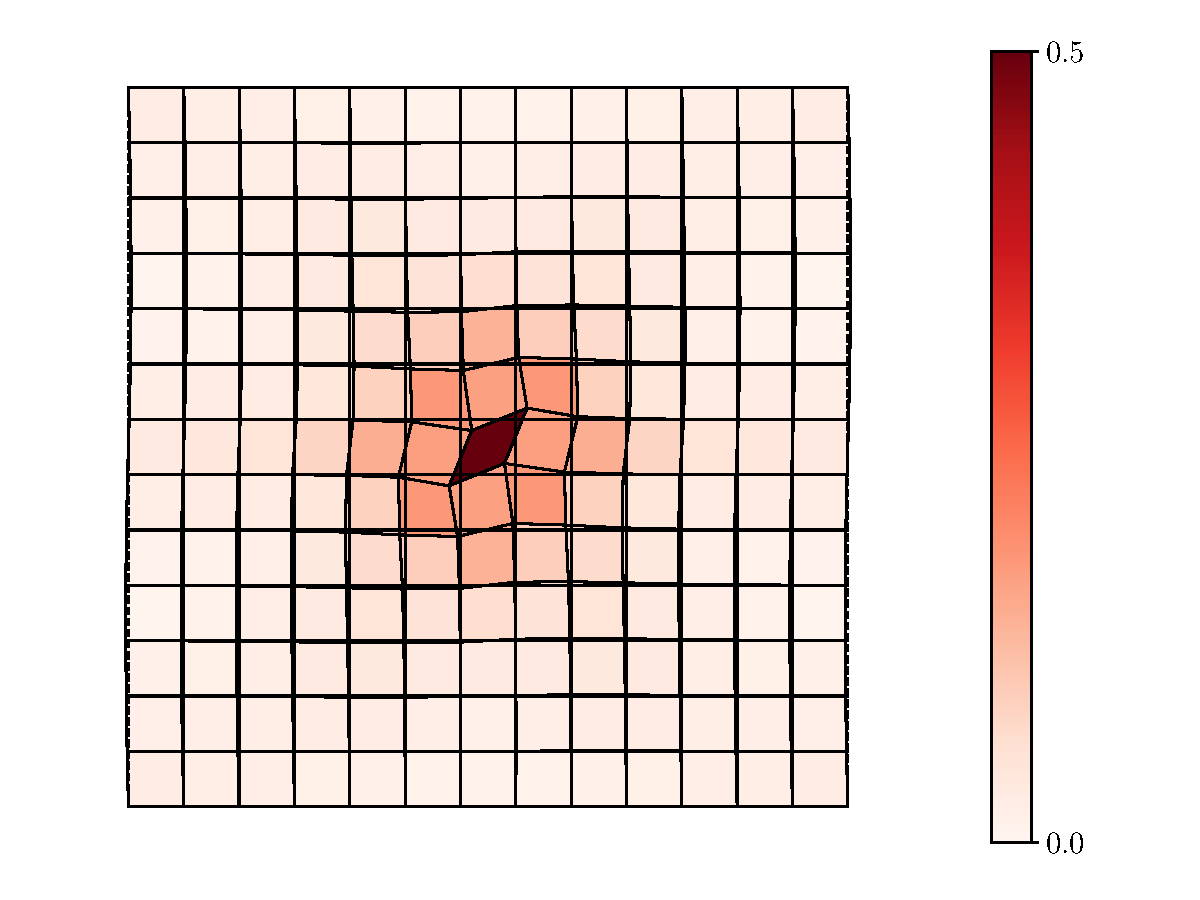
\includegraphics[width=\textwidth]{perturbation_simple-shear.pdf}
        \subcaption{Simple shear}
        \label{fig:perturbation:simple-shear}
    \end{minipage}
    \hfill
    \begin{minipage}[t]{.49\textwidth}
        \centering
        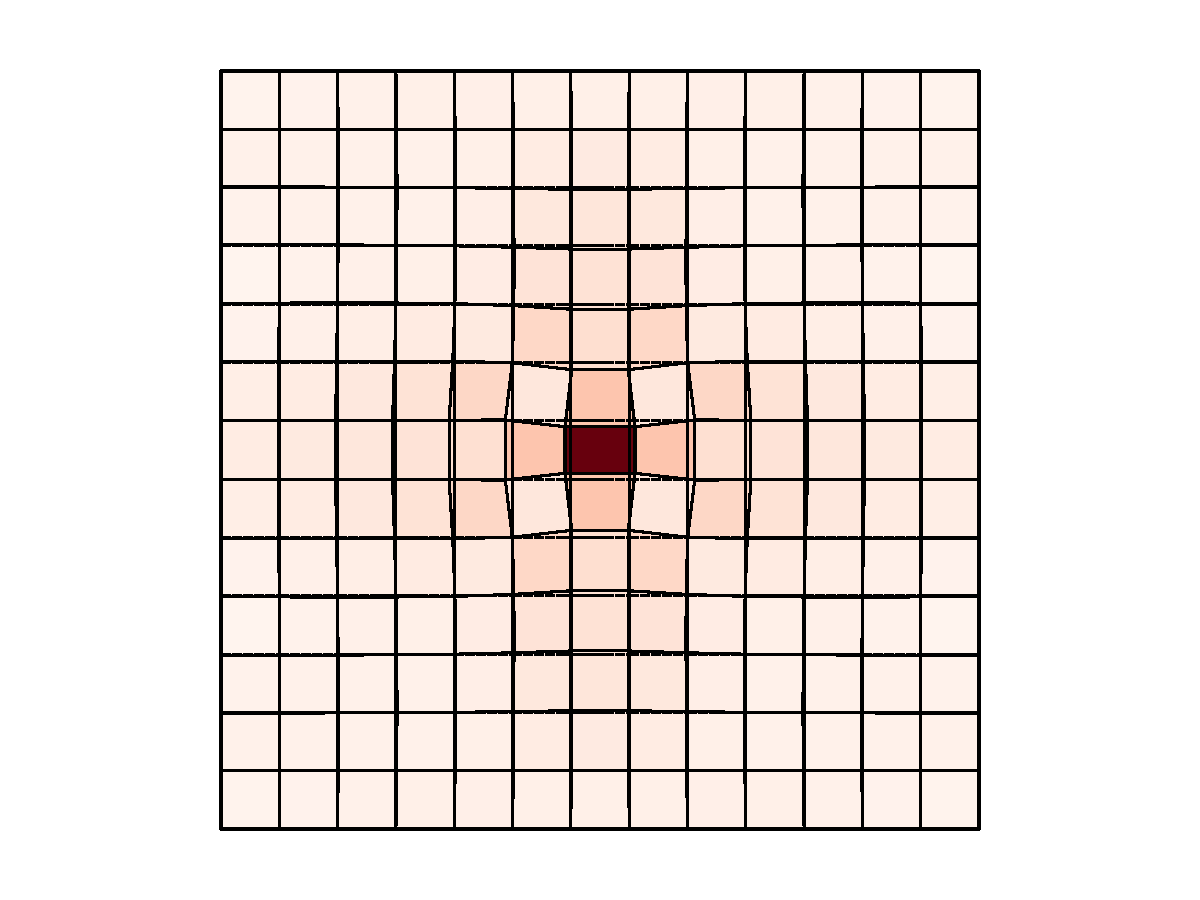
\includegraphics[width=\textwidth]{perturbation_pure-shear.pdf}
        \subcaption{Pure shear}
        \label{fig:perturbation:pure-shear}
    \end{minipage}
    \caption{
        Perturbation modes.
        The shown colour is the equivalent stress resulting from the perturbation.}
    \label{fig:perturbation}
\end{figure}

\begin{figure}[htp]
    \centering
    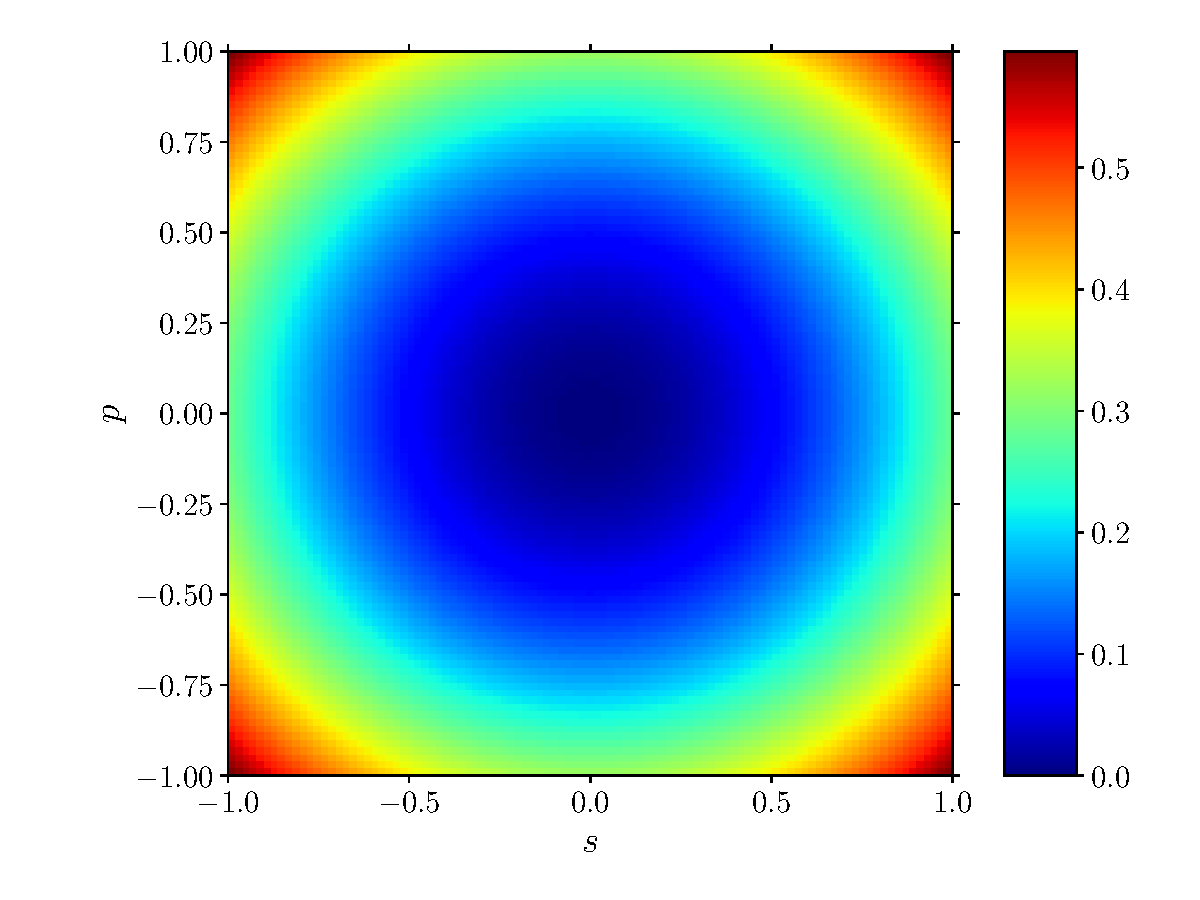
\includegraphics[width=.5\textwidth]{phase-diagram_energy.pdf}
    \caption{
        Energetic cost of a perturbation with a linear combination of the two
        perturbation modes:
        $\bm{\sigma}^* = p \bm{\sigma}^*_p + s \bm{\sigma}^*_s$.}
    \label{fig:energy}
\end{figure}

\begin{figure}[htp]
    \centering
    \captionsetup[subfigure]{justification=centering}
    \begin{minipage}[t]{.49\textwidth}
        \centering
        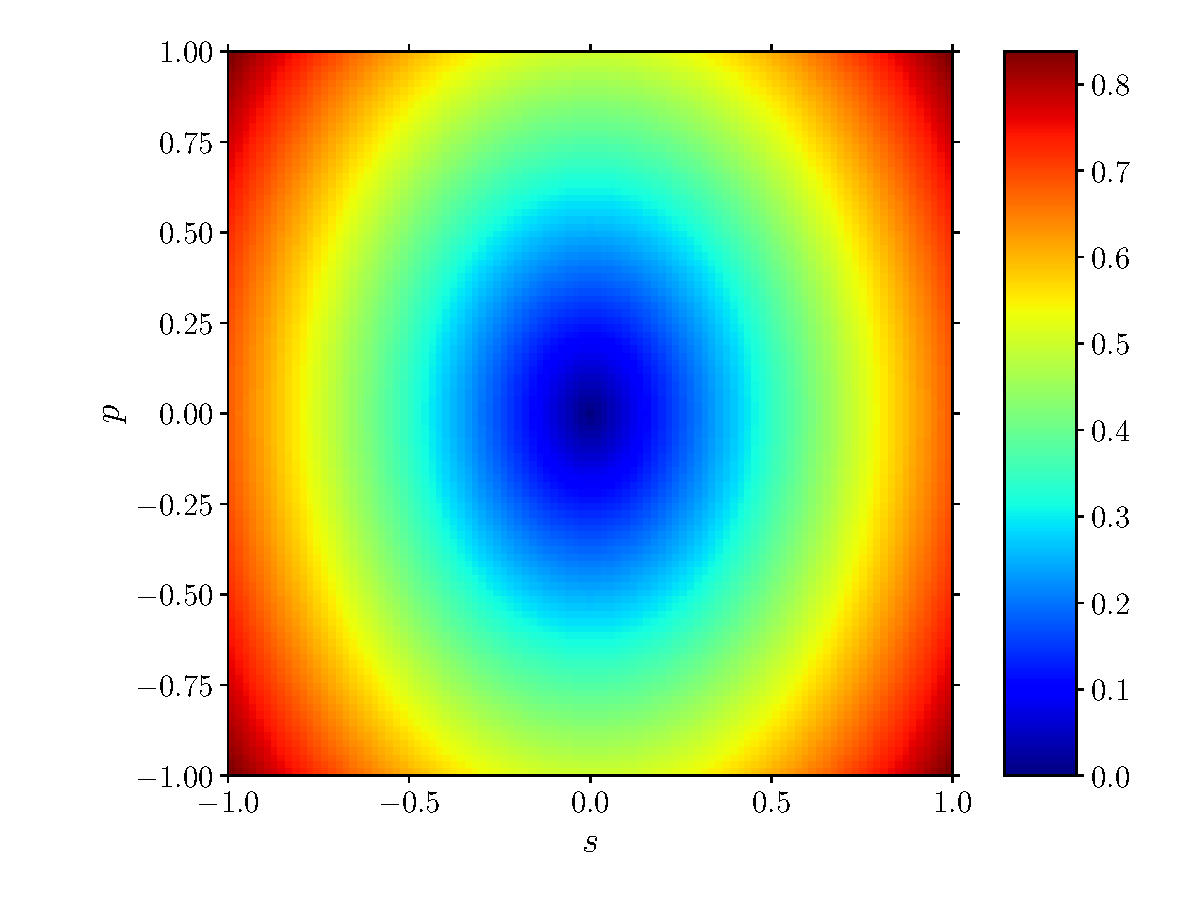
\includegraphics[width=\textwidth]{phase-diagram_sig.pdf}
        \subcaption{
            Equivalent stress.
        }
        \label{fig:phase-diagram:sig}
    \end{minipage}
    \hfill
    \begin{minipage}[t]{.49\textwidth}
        \centering
        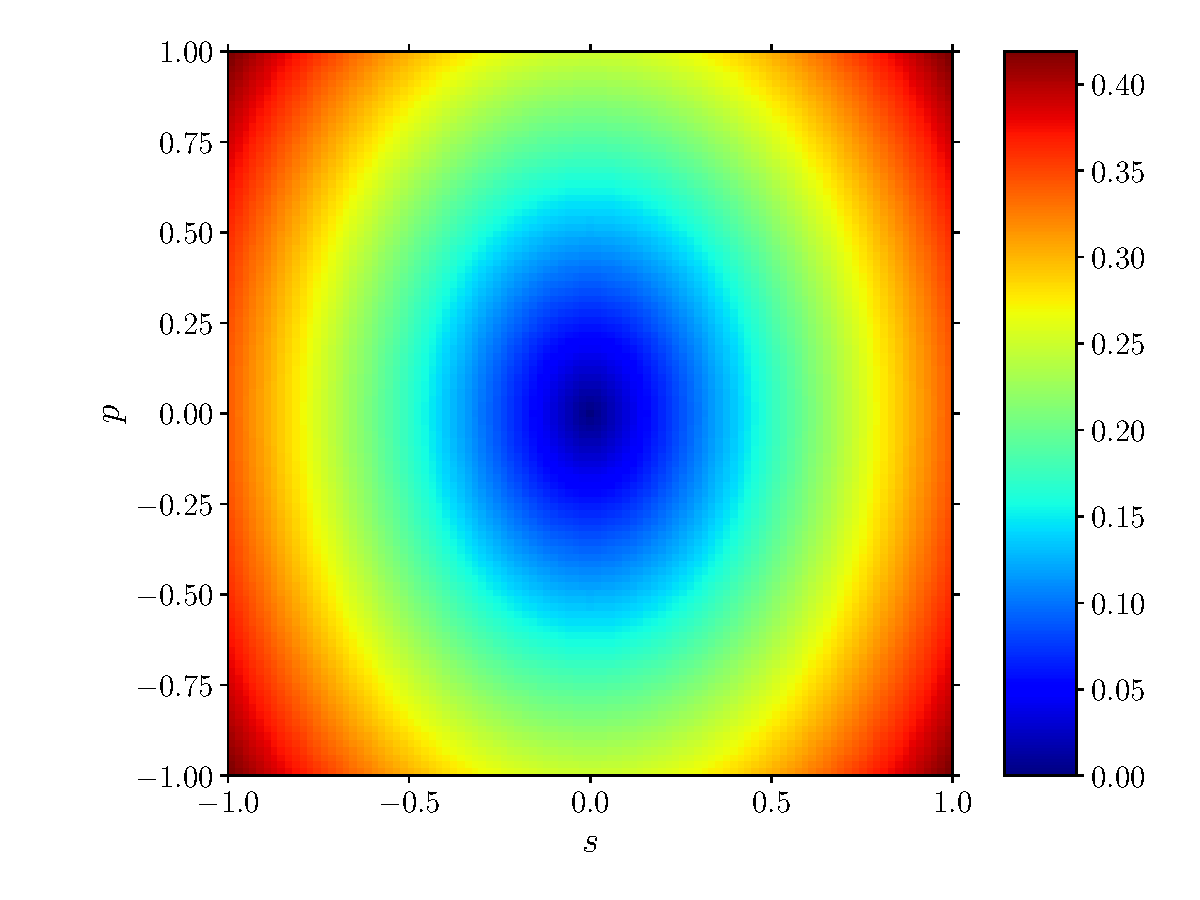
\includegraphics[width=\textwidth]{phase-diagram_eps.pdf}
        \subcaption{
            Equivalent strain.
        }
        \label{fig:phase-diagram:eps}
    \end{minipage}
    \caption{
        Resulting
        \subref{fig:phase-diagram:sig} equivalent stress and
        \subref{fig:phase-diagram:eps} equivalent strain
        for a perturbation with a linear combination of the two perturbation modes:
        $\bm{\sigma}^* = p \bm{\sigma}^*_p + s \bm{\sigma}^*_s$.
    }
    \label{fig:phase-diagram}
\end{figure}

\end{document}
